\section{Results} \label{sec:results}
This section presents the main results for both Newton and Broyden methods. The initial guess and number of iterations vary according to the system of equations but are the same for both methods. Tolerance is set to $10^{-15}$ for both examples.

\subsection{First Nonlinear System}
The first nonlinear system given Eq. \eqref{eq:Sys1} uses  $x_0 = \{0.1, 0.1\}$ as the initial guess, and has 10 iterations for both methods. Table \ref{tab:Sys1} presents the results for the first system using Newton and Broyden methods.
\begin{table}[H]
    \centering
    \caption{Results for the first nonlinear system}
    \begin{tabular}{cccc}
        \hline
        \multicolumn{4}{c}{\textbf{Newton's Method}} \\ \hline
        Iteration & $x$ & $y$ & residual\\
        \hline
        0 & 0.1 & 0.1 & 0.43736 \\
        1 & 0.4627600085 & 0.0734399488 & 0.18007 \\
        2 & 0.3969527820 & 0.0354011946 & 0.00917 \\
        3 & 0.3938604085 & 0.0321511366 & 2.88e-05 \\
        4 & 0.3938494529 & 0.0321427390 & 2.910e-10 \\
        5 & 0.3938494528 & 0.0321427389 & 2.220e-16 \\ \hline
        \multicolumn{4}{c}{\textbf{Broyden's Method}} \\ \hline
        Iteration & $x$ & $y$ & residual\\
        0 & 0.1 & 0.1 & 0.43736 \\
        1 & 0.4627600085 & 0.0734399488 & 0.18007 \\
        2 & 0.3856395478 & 0.0055231374 & 0.04633 \\
        3 & 0.3902269923 & 0.0344443408 & 0.00631 \\
        4 & 0.3941767806 & 0.0314940531 & 0.00083 \\ 
        5 & 0.3938644022 & 0.0321212671 & 3.09e-05 \\
        6 & 0.3938492796 & 0.0321429715 & 3.47e-07 \\
        7 & 0.3938494532 &  0.032142738 & 8.49e-10 \\
        8 & 0.3938494528 & 0.0321427389 & 6.84e-13 \\
        9 & 0.3938494528 & 0.0321427389 & 1.11e-16 \\ \hline
    \end{tabular}
    \label{tab:Sys1}
\end{table}

Figure \ref{fig:Sys1} depicts the convergence for both methods. Newton's method converges in 5 iterations, while Broyden's takes almost the double, 9 iterations. Both methods achieve the same solution, $x = 0.3938494528$ and $y = 0.0321427389$, with a residual of the order of $10^{-16}$.
\begin{figure}[H]
    \centering
    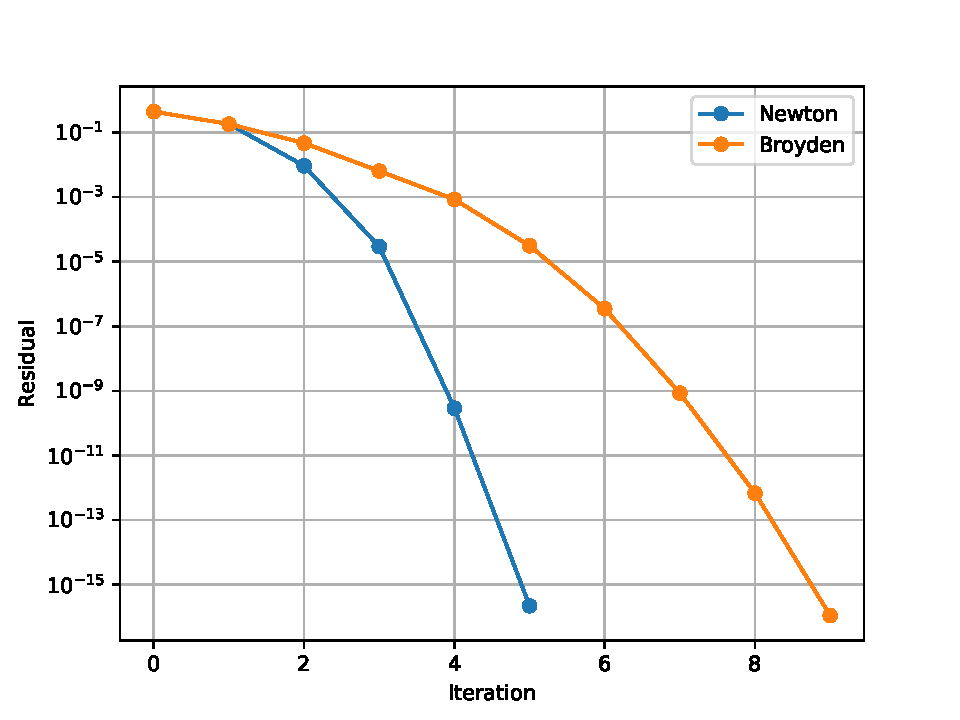
\includegraphics[width=0.7\textwidth]{Residual1.pdf}
    \caption{Convergence for the first nonlinear system}
    \label{fig:Sys1}
\end{figure}

\subsection{Second Nonlinear System}
The second nonlinear system given Eq. \eqref{eq:Sys2} uses  $x_0 = \{0.1, 0.1, 0.1\}$ as the initial guess, and has 30 iterations for both methods. Table \ref{tab:Sys2} presents the results for the second system using Newton and Broyden methods.
\begin{table}[H]
    \centering
    \caption{Results for the second nonlinear system.}
    \begin{tabular}{ccccc}
        \hline
        \multicolumn{5}{c}{\textbf{Newton's Method}} \\ \hline
        Iteration & $x$ & $y$ & $z$ & Residual\\
        \hline
        0 & 0.1 & 0.1 & 0.1 & 2.32838 \\
        1 & -0.98379345166 & 2.2156661291 & 1.88681273224 & 5.74369\\
        2 & 1.39885410699 & 2.0132350005 & -1.29854408331 & 4.07938\\
        3 & 3.15367430755 & 1.73619021977 & -3.96154226685 & 39.75890\\
        4 & 2.58232829725 & 1.92098936848 & -3.06620946128 & 11.63550\\
        5 & 2.20584340512 & 2.02126203014 & -2.49633866143 & 2.78584\\
        6 & 2.04009533921 & 2.07754843321 & -2.2477262380 & 0.36281\\
        7 & 2.01019345695 & 2.09121239898 & -2.2041500598 & 0.00896\\
        8 & 2.00936979322 & 2.0917047033 & -2.20300865265 & 5.50e-06\\
        9 & 2.00936923461 & 2.09170513415 & -2.2030079444 & 1.81e-12\\
        10 & 2.00936923461 & 2.0917051341 & -2.20300794446 & 4.44e-16\\
        \hline
    \end{tabular}
\end{table}
\begin{table}[H]
    \ContinuedFloat
    \centering
    \caption{Results for the second nonlinear system (continued).}
    \begin{tabular}{ccccc}
        \hline
        \multicolumn{5}{c}{\textbf{Broyden's Method}} \\ \hline
        Iteration & $x$ & $y$ & $z$ & Residual\\
        0 & 0.1 & 0.1 & 0.1 &  \\ 
        1 & -0.98379345166 & 2.2156661291 & 1.88681273224 & 2.32838\\
        2 & -2.86800321300 & -0.736524949 & 5.02933927946 & 5.74369\\
        3 & -0.96629288250 & -0.639022704 & 1.14171550902 & 9.38550\\
        4 & -1.14214386855 & -0.772153622 & 1.19899623589 & 0.32993\\
        5 & -1.27546528568 & -1.086899010 & 0.80710460716 & 0.64812\\
        6 & -1.06426239703 & -0.520529040 & 1.50883577012 & 1.56098\\
        7 & -1.06810147286 & -0.383391728 & 1.63192385971 & 0.20765\\
        8 & -1.05115463611 & -0.351985295 & 1.63848950012 & 0.10285\\
        9 & -1.00884044531 & -0.111511495 & 1.84570543100 & 0.04046\\
        10 & -1.04138584935 & -0.224753681 & 1.75881524320 & 0.11954\\
        11 & -1.01392825338 & 0.3424018291 & 2.29684285546 & 0.03378\\
        12 & -1.03006301317 & -0.094337434 & 1.89731370887 & 0.10673\\
        13 & -1.02203741634 & 0.0573997855 & 2.05329309938 & 0.07035\\
        14 & -0.99440018782 & 0.7406037349 & 2.75706745631 & 0.06132\\
        15 & -1.02471257131 & 0.1091210711 & 2.10797608681 & 0.58571\\
        16 & -1.02143379112 & 0.1486759010 & 2.15081073230 & 0.03928\\
        17 & -1.02190742245 & 0.2041423038 & 2.20724613288 & 0.02584\\
        18 & -1.01907494179 & 0.2027702169 & 2.20770475416 & 0.00591\\
        19 & -1.02102506714 & 0.1970132648 & 2.20050276823 & 0.00215\\
        20 & -1.02025912697 & 0.1996163781 & 2.20366469063 & 0.00143\\
        21 & -1.02025768870 & 0.1996113540 & 2.20365643426 & 1.09e-05\\
        22 & -1.02025684824 & 0.1995979744 & 2.20363943856 & 4.50e-06\\
        23& -1.020257309945 & 0.1996053765 & 2.20364884435 & 5.57e-06\\
        24 & -1.02025730998 & 0.1996053775 & 2.20364884555 & 6.70e-10\\
        25 & -1.02025730998 & 0.1996053775 & 2.20364884553 & 1.61e-13\\
        26 & -1.02025730998 & 0.1996053775 & 2.20364884553 & 3.30e-16\\ 
        \hline
    \end{tabular}
    \label{tab:Sys2}
\end{table}

Figure \ref{fig:Sys2} shows the convergence for both methods. Newton's method converges in 10 iterations, while Broyden's takes 26 iterations. Differently from the first system, the methods do not converge to the same solution. Newton's method converges to $x = 2.00936923461$, $y = 2.0917051341$, and $z = -2.20300794446$, while Broyden's method converges to $x = -1.02025730998$, $y = 0.1996053775$, and $z = 2.20364884553$. Regardless of the achieved solution, the residuals are of the order of $10^{-16}$ for both methods.
\begin{figure}[H]
    \centering
    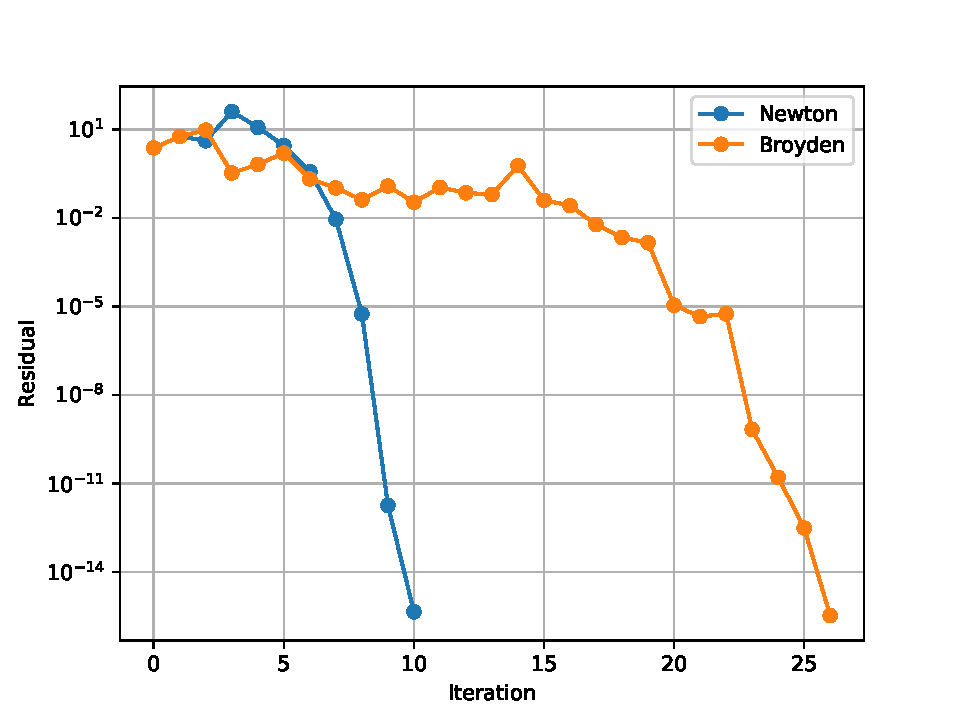
\includegraphics[width=0.7\textwidth]{Residual2.pdf}
    \caption{Convergence for the second nonlinear system}
    \label{fig:Sys2}
\end{figure}

Both solutions are easily verified by substituting the values into the system of equations. 